\chapter{Toward an Evaluation Platform for Inductive Model Synthesis\label{chapter:stamina}}

A grammar induction algorithm is commonly evaluated by reporting an accuracy measure of the model it learns for increasing sizes of the training sample. This has been done in the previous chapter for example, where plots illustrate the convergence of QSM and ASM toward a ``good'' model when the training sample -- or more generally their input -- becomes rich enough. This kind of setup can also be used to make different induction techniques compete, by evaluating them on common benchmarks of increasing difficulty for instance. In that respect, the Abbadingo contest have had a notable impact~\cite{Lang:1998}. Among others indeed, the competition triggered the discovery of the evidence-driven state merging heuristics used by Blue-Fringe and QSM. Since the end of the competition, it has been frequently used as a reusable benchmark and evaluation protocol for grammar induction (see e.g.~\cite{Lucas:2003, Bongard:2005, Lucas:2005, Adriaans:2006, Dupont:2008, Lambeau:2008, Heule:2010}).

A weakness of the Abbadingo benchmark, however, is that it only contains induction problems for automata defined on alphabets of two letters only. Freezing certain parameters, here the alphabet size, is necessary for keeping a competition sufficiently simple and understandable for its participants. Nevertheless, a side effect is that it limits the generalization of the conclusions drawn from competition results but also the re-usability of the competition protocol itself. 

This effect has been clearly observed when conducting evaluations reported in this thesis. On one side, reusing Abbadingo allows situating and comparing our results with previous ones, and to do so on a sound and agreed benchmarking protocol. On the other side, limiting evaluations to binary alphabets is arguable from a software engineering point of view, mainly because even small behavior models are commonly defined on thirty events or more. Therefore, one could question the representativeness of synthetic machines and samples used in the previous chapter for capturing certain characteristics of behavior models. 

Unfortunately, modifying the Abbadingo protocol to take larger alphabets into account appears more difficult than one could expect. Indeed, many of its components -- automata and samples generators, in particular -- strongly rely on (sometimes subtle) assumptions related to the use of a binary alphabet. All these reasons have led us to build an alternative benchmark, called Stamina (for \emph{State Machine Inference Approaches}), which builds on and extends Abbadingo but focuses on the complexity of the learning with respect to the alphabet size. Among others, our protocol relies on adapted procedures for generating automata and samples that better fit characteristics of behavior models encountered in the software engineering community.

To draw community's attention to the influence of the alphabet size on the difficulty of the learning task (an aspect that has not been tackled in previous competitions or benchmarks) and to federate ideas about machine learning applied to behavior synthesis, Stamina has initially taken the form of an induction competition, in a similar spirit to Abbadingo. The competition has officially ran between March and December 2010 and was organized in collaboration with the universities of Sheffield and Leicester, and officially sponsored by the Engineering and Physical Sciences Research Council\footnote{http://www.epsrc.ac.uk/}. The winning algorithm DFASAT, as well as a few additional competitors, have significantly outperformed the Blue-fringe baseline on a variety of problems. DFASAT mixes SAT solving and state merging and, among other ingredients, uses a new scoring heuristics that proved especially useful to infer the kind of state machines considered in the competition. In addition to pushing forward the state-of-the-art of the induction problem, the competition triggered interest from at least three communities, namely Machine Learning, Software Engineering and Formal Methods. The Stamina website\footnote{http://stamina.chefbe.net/} is still available and has been updated to serve as an online benchmark and evaluation platform for model synthesis instead of a formal competition.

This chapter is organized as follows. Section~\ref{section:stamina-background} provides background on Abbadingo and discusses its weaknesses for evaluating inductive model synthesis techniques. The detailed setup of Stamina is explained in section~\ref{section:stamina-setup}. Section~\ref{section:stamina-results} presents the main results of the competition and also includes a description of the winning technique. We close this chapter in Section~\ref{section:stamina-platform}, which describes the changes we made to let the competition server evolve to an evaluation platform and summarizes future work along this direction.

\section{Objectives\label{section:stamina-background}}

\subsection{Background on the Abbadingo contest\label{subsection:stamina-abbadingo}}

Abbadingo is designed as a grid of 16 induction problems. A competing learner is provided a set of training strings labeled as positive or negative by an unseen DFA and is required to predict the labels that the DFA would assign to a set of testing strings. The 16 problems are classified in a grid of two difficulty dimensions. The first one is the size of the target automata, as the number of its states (64, 128, 256 or 512). The second is the sparsity of the training sample, in terms of four sparsity levels. These levels have been tuned by manually inspecting learning curves of the Trakhenbrot-Barzdin algorithm. Indeed, the latter was a state-of-the-art induction algorithm in 1997. Therefore, the problem grid has been adjusted in such a way that it solves the four problems with largest samples.

Target automata, training and test strings of Abbadingo have all been drawn from uniform random distributions. Random automata have been generated by constructing and minimizing degree-2 directed graphs (as a consequence of using a binary alphabet), edges and states labels (final or not) having been chosen by flipping a fair coin. To keep the generation of the training set sufficiently simple, only automata of depth of exactly $2log_2(n)-2$ have been kept for inclusion in the problem grid. A training set for a target of size $n$ is made of a random sample drawn without replacement from a uniform distribution over the collection of $16n^2 -1$ binary strings whose length lies between 0 and $2log_2(n)+3$ inclusively. This latter bound has been chosen to have a good chance of reaching the deepest state of the automaton, a necessary criteria toward a structurally complete sample, which is not guaranteed though. A testing set consists in 1800 strings drawn from the remaining strings. As a consequence, training and test sets do not overlap.

The testing protocol of Abbadingo consists in the learner labeling each string of the test set and submitting this labeling to an online oracle\footnote{available at http://abbadingo.cs.nuim.ie/}. To avoid hill climbing -- where the feedback of the competition server could be used by the learner to iteratively optimize a first solution -- this oracle only provides a single bit of feedback which tells whether or not the problem is broken. A problem is considered broken if the accuracy (computed as the proportion of the 1800 test strings correctly labeled), of the labeling is at least 99\%. During the competition itself, the first participant to break a given problem gained credit for it. Abbadingo allowed multiple winners by defining a partial order on problem difficulty: a problem $A$ is considered harder than a problem $B$ if its DFA has more states \emph{and} its training sample is sparser. 

Two winners, Rodney Price and Hugues Julli\'e, won the competition with similar algorithms relying on what has since been called \emph{evidence driven state merging} (EDSM). This term captures the strategy of first performing state merges that are supported by the most evidence, according to a specific scoring heuristics. Among other contributions, the competition has helped finding a good scoring heuristics based on the number of final states merged during the determinization process. Mixing this evidence driven idea with the red-blue merge order described previously (see chapter~\ref{chapter:inductive-synthesis}) leads to the particularly fast and simple algorithm known as \emph{Blue-fringe}, for which the post-analysis Abbadingo paper provides a reference description~\cite{Lang:1998}.

\subsection{Weaknesses for evaluating inductive model synthesis}

Since the end of the competition, Abbadingo has evolved to become a reusable protocol and online benchmark for induction techniques. To situate and compare our results, the evaluations proposed in chapter~\ref{chapter:inductive-synthesis} of the present thesis have been precisely conducted on a similar protocol. However, the fact that Abbadingo fixes the size of the alphabet to only two letters limits the relevance of reusing its protocol for evaluating behavior model synthesis techniques. This is mainly because behavior models are commonly defined on larger sets of events. As an example, the small phone case-study studied in the previous chapter already uses 16 distinct events for a state machine of only 23 states. Strictly speaking, the weakness is not the small alphabet size itself but has to be found in the impact of using binary alphabets on the different artifacts required for building such a benchmark:

\begin{description}
\item[Automata] The automata randomly generated by Abbadingo have a small, quasi-constant, state degree (number of incident edges). This is a consequence of using binary alphabets: due to the its deterministic nature, an automaton of $n$ states has at least $n$ and at most $2n$ edges; these edges are uniformly distributed over all states. 

In contrast, automata modeling software systems involve transitions that may be triggered by any of a large number of events (mouse clicks, function names IO events, etc.). The number of outgoing transitions for a given state can be very large and vary significantly from state to state. A review of the state machines found in the literature shows that while most states have in- and out-degrees of one or two transitions, state machines tend to contain a small proportion of states with a high in-degree (e.g. those modeling exception handling) or a high out-degree (an \emph{idle} state where a software agent waits for external stimuli in terms of input events). Other states are \emph{sink} accepting states, that is, they have an out-degree of 0 (explicit modeling of the ability of a system to halt)~\cite{Walkinshaw:2008}.

The automata generated with the Abbadingo procedure do not present such characteristics, due to the small alphabet size. Moreover, because of the uniform edge distribution it implies, this procedure would not naturally lead to automata presenting the characteristics aforementioned even if it was adapted for handling larger alphabets.

\item[Samples] Abbadingo samples are simply drawn from uniform random distribution over the collection of all (binary) strings up to a prescribed length. The target machine is used to classify them as positive or negative. For statistical reasons, the respective number of positive and negative strings is naturally balanced.

Unfortunately, this procedure is no longer viable when working with larger alphabets (unless state machines present similar characteristics to the ones of Abbadingo, which is not the case, as previously discussed). Indeed, in this case an overwhelming majority of random sequences in $\Sigma^*$ are negative. Moreover, the few positive strings that would be made available would probably not provide a sufficient coverage of the target machine for obtaining good induction results (see Section~\ref{section:inductive-background}).

\item[Scoring] The choice of the accuracy measure (defined in Abbadingo as the proportion of test strings that are correctly classified by the automaton learned) is also arguable if one relaxes the assumption of having balanced test samples~\cite{Walkinshaw:2008}. In the extreme case of a test set largely overwhelmed by negative strings for example, a learner classifying all strings as negative would still obtain a comfortable score. A better measure should consider the acceptance of positive strings and the rejection of negative ones equally important. 
\end{description}

As shown, conducting sound evaluations without making the assumption of a binary alphabet requires rethinking important parts of the underlying protocol. To capitalize over and share the cost of such a work we designed Stamina as both a public complement and an alternative to Abbadingo. Focusing on characteristics of behavior models, it is also a call to cross-fertilization between the machine learning and software engineering communities. To achieve this goal in a fun way, Stamina first took the form of an online induction competition before evolving to an online benchmark, in a similar spirit to Abbadingo. The next section details the Stamina setup as designed for the competition. Changes made to the platform since the end of the competition will be explained in Section~\ref{section:stamina-platform}.

%%%%%%

\section{Stamina setup\label{section:stamina-setup}}

The competition scenario chosen for Stamina is very similar to the one of Abbadingo: 

\begin{quotation}
A learner downloads a training set made of positive and negative strings, infers a model using her induction technique, uses it to label strings of a test sample and finally, submits these labels to the competition server. The latter scores the submission and provides a binary feedback, according to whether the problem is considered broken or not.
\end{quotation}

If the competition scenario is similar, Stamina differs from Abbadingo in that it focuses on the complexity of the learning with respect to the alphabet size, and therefore relies on an adapted generation protocol for target automata and samples. The next sections details the choices that have been made and the key differences with Abbadingo.

\subsection{Competition grid}

As in Abbadingo, induction problems are classified in a grid. Here, the competition grid is divided in cells of five problems each, where each cell corresponds to a particular combination of sparsity and alphabet size. Table~\ref{stamina:table:problem-grid} shows how problems are distributed in cells. Easier problems (with a smaller alphabet and a larger sample) are toward the upper-left of the table, and the harder problems (larger alphabet and smaller sample) are toward the bottom-right.

\begin{table}[h]
\begin{center}
\begin{tabular}{c|c c c c}
&\multicolumn{4}{|c}{Sparsity}\\ 
\textbf{$|\Sigma|$} & \textbf{100\%} & \textbf{50\%} & \textbf{25\%} & \textbf{12.5\%}\\
\hline
\textbf{2}  & 1-5   & 6-10  & 11-15 & 16-20 \\
\textbf{5}  & 21-25 & 26-30 & 31-35 & 36-40 \\
\textbf{10} & 41-45 & 46-50 & 51-55 & 56-60 \\
\textbf{20} & 61-65 & 66-70 & 71-75 & 76-80 \\
\textbf{50} & 81-85 & 86-90 & 91-95 & 96-100\\
\end{tabular}
\end{center}
\caption{\label{stamina:table:problem-grid}Grid of 100 problems distributing the induction difficulty among two dimensions: sparsity of the learning sample and alphabet size.}
\end{table}

\noindent Similarities and differences with Abbadingo are:

\begin{itemize}

\item An increasing size of the alphabet forms a first difficulty dimension, ranging from 2 to 50 letters. The lower bound allows comparing results with Abbadingo on easiest problems while the upper bound is representative of behavior models found in the literature.

\item Unlike Abbadingo in which the varying automaton size is a difficulty dimension (ranging from 64 to 512), Stamina only considers automata of roughly 50 states. By contrast, these automata present characteristics of behavior models in terms of the variance of their state degree, among other differences (see section~\ref{subsection:stamina-machines})

\item The second difficulty dimension, the decreasing size of the training sample, is similar to Abbadingo. Nevertheless, samples in Stamina are generated ``from the machine'' by a random walk procedure, instead of randomly drawn from all possible strings (see section~\ref{subsection:stamina-samples}).

\item Instead of an accuracy measure, submissions in Stamina are scored using a \emph{binary classification rate} (BCR). BCR places an equal emphasis on the accuracy of an inferred model in terms of acceptance of positive sequences and rejection of negative ones. Obtaining a BCR score of at least 99\% is required to consider a problem broken. A cell is broken if its five problems are broken by the same learner (see section~\ref{subsection:stamina-scoring})

\item Unlike Abbadingo, Stamina allowed only one winner, being the first learning technique to break a hardest cell among those broken in the competition. To adjust the grid and choose cell difficulties, Blue-fringe has been scored on each problem (see section~\ref{subsection:stamina-baseline}). An implementation of this baseline algorithm is available for download.

\end{itemize}

\subsection{State Machines\label{subsection:stamina-machines}}

In order to generate state machines, a quick review of software models has been conducted. Observations have been made on a small sample (about 20 systems) of case-study models found in research publications. State machine models were analyzed in terms of their states, transitions, alphabet sizes, in-/out degree and depth. Although the sample is too small to form any authoritative conclusions, findings can be interpreted as being indicative. Following these observations, Stamina machines have been generated using a variant of the Forest-Fire algorithm~\cite{Leskovec2007}. The algorithm has been tuned to generate state machines presenting the following characteristics:

\begin{description}

\item[Number of states] All state machines have approximately 50 states. Although somewhat larger than the conventional state machines identified in the literature, this is to ensure that a well-performing technique could scale to infer models for reasonably complex software systems. Also, is has been decided not to consider state machines of exactly 50 states to avoid introducing a strong bias in the benchmark. Automaton sizes range from 41 to 59 states with an uniform distribution. Note that this latter information was not disclosed during the competition.

\item[Accepting ratio] A roughly equal proportion of accepting and rejecting states has been chosen, a feature is shared with Abbadingo. While most software models, and LTS in particular, have all accepting states it has been decided to keep non accepting states as well. Doing so keeps our setup sufficiently close to former ones and, in particular, avoids restricting the problem to the inference of prefix-closed regular languages. As discussed in Section~\ref{section:inductive-background}, inferring prefix-closed languages looks an easier problem than general regular inference. Hence, a competition winner would be expected to perform equally well, if not better, when inferring machines with all accepting states.

\item[Degree distribution] Following observations from the literature, state machines present an important variance of their state degree, especially on largest alphabets. Also, they may have sink accepting states, that is, states with no outgoing transition.

\item[Deterministic and minimal] Following common setup of regular inference experiments, all Stamina machines are both deterministic and minimal.

\end{description}

\subsection{Training and test samples\label{subsection:stamina-samples}}

Training and test samples have been generated using a dedicated generation procedure. This procedure aims at simulating the way examples of system behavior are usually obtained in the software engineering community (e.g. a collection of program traces at an implementation level, the generation of scenarios at a design level, and so on). Stamina samples present the following characteristics:

\begin{description}

\item[Generated by the target] A dedicated algorithm has been implemented to generate positive strings by walking through the automaton. From the initial state it randomly selects outgoing transitions with an uniform distribution. When an accepting state $v$ is reached, the generation ends with a probability of $1.0/(1 + 2*outdegree(v))$. This procedure simulates an ``end of string'' transition from state $v$ with half the probability of an existing transition. The length distribution of the strings generated is approximately centered on $5 + depth(automaton)$. As in Abbadingo, this provides a good chance of reaching the deepest state of the automaton. However, no guarantee is given of having a structurally complete sample.

\item[Negative strings] Negative strings are generated by randomly perturbing positive strings. Three kinds of edit operation are considered: substituting, inserting, or deleting a symbol. The editing position is randomly chosen according to an uniform distribution over the string length. Substitution and insertion also use an uniform distribution over the alphabet. The number of editing operations is chosen according to a Poisson distribution (with a mean of 3) and the three editing operations have an equal change of being selected. The randomly edited string is included in the negative sample provided that it is indeed rejected by the target machine. Otherwise, it is simply discarded.

\end{description}

The random walk algorithm and perturbation procedure serve as building blocks for the generation of training and test samples for each problem. Using them, a set of 20.000 strings is first sampled from the target machine. This sample contains roughly equal number of positive and negative strings and usually contains duplicates. The distinct strings of the initial sample are then equally partitioned into two sets, taking care of respecting the positive and negative balance in each one. The first set is used to generate the test sample, the second one to generate the learning sample. The test sample contains 1500 strings randomly drawn without replacement from the first set. It never contains duplicates, to avoid favoring repeated strings in the scoring metric. The official training sets are sampled from the second set with different levels of sparsity (100\%, 50\%, 25\%, 12.5\%) and usually contain duplicates, as a consequence of the random walk generation from the target machine. As a consequence of this procedure, training and test sets do never intersect.

\subsection{Submission and Scoring\label{subsection:stamina-scoring}}

Solutions to Stamina problems must be submitted as binary strings to the competition server\footnote{available at http://stamina.chefbe.net}. For this, the learner is expected to produce a binary sequence of labels where, for each test string, a $1$ is added to the sequence if the string is considered to be accepted, and a $0$ otherwise. To establish the solution accuracy, the sequence is compared to a reference string representing the correct labeling of the test set by the target model. The overlap between the two binary strings is measured with the \emph{balanced classification rate (BCR)}. The harmonic BCR measure is chosen because it places an equal emphasis on the accuracy of the inferred model in terms of the acceptance of positive sequences and the rejection of negative ones. Also, it does not require the test set to be balanced in terms of number of positive and negative sequences. 

Harmonic BCR is the harmonic mean of two factors. $Sensitivity$ is the proportion of positive matches that are predicted to be positive and $Specificity$ is the proportion of true negatives that are predicted to be negative. Conventionally, BCR is simply computed as the arithmetic mean of sensitivity and specificity, but the harmonic mean is preferred here because it favors balance between the two. So in terms of the sets of true and false positives and negatives ($TP$, $FP$, $TN$ and $FN$),

$$Sensitivity=\frac{|TP|}{|TP \cup FN|}$$ 

$$Specificity=\frac{|TN|}{|TN \cup FP|}$$

$$BCR=\frac{2*Sensitivity*Specificity}{Sensitivity + Specificity}$$

As in Abbadingo, hill-climbing is made almost impossible by a binary feedback from the oracle, according to whether the problem is broken or not. For recall, a problem is considered broken if the BCR score obtained is greater than or equal to 0.99. A cell is considered broken if all of its five problems are broken. The Stamina website dedicates a private section to  each registered participant that provides visual feedback about the performance of her algorithm(s). In this section, problems and cells of the submission grid turn to green when broken.

\subsection{Blue-fringe baseline\label{subsection:stamina-baseline}}

Blue-fringe has been ran on all Stamina problems, first to adjust the grid for guaranteeing the feasibility of the competition and second, to fix the difficulty level of each cell, on which the winning criteria relies.

Adjusting the grid is similar in spirit to what has been done for Abbadingo. The idea is to adjust free parameters (actual sizes of the training and test sets, average length of the strings with respect to the automaton depth, and so on) in such a way that the state-of-the-art algorithm, here Blue-fringe, breaks the easiest problems. This trial-and-error process converged with three problems broken in the easiest cell (therefore not itself broken) and reasonable scores for the two remaining problems as well as those of adjacent cells.

The performance of the baseline is summarized in Table~\ref{table:stamina-baseline} and illustrated with convergence curves in Fig.~\ref{stamina:image:bluefringe-performance}. As shown, the BCR score decreases along each of the two difficulty dimensions, experimentally confirming the expected effect of an increasing alphabet size on the induction difficulty. 

\begin{table}
\begin{center}
\begin{tabular}{c|c c c c}
&\multicolumn{4}{|c}{\textbf{Sparsity}}\\ 
\textbf{$|\Sigma|$} & \textbf{100\%} & \textbf{50\%} & \textbf{25\%} & \textbf{12.5\%}\\
\hline
\textbf{2}  & 0.99 (1) & 0.95 (1) & 0.67 (3) & 0.66 (3)\\
\textbf{5}  & 0.97 (1) & 0.78 (2) & 0.59 (4) & 0.52 (4)\\
\textbf{10} & 0.93 (1) & 0.64 (3) & 0.51 (4) & 0.50 (4)\\
\textbf{20} & 0.91 (1) & 0.63 (3) & 0.54 (4) & 0.51 (4)\\
\textbf{50} & 0.81 (2) & 0.64 (3) & 0.57 (4) & 0.50 (4)\\
\end{tabular}
\end{center}
\caption{Average BCR of Blue-fringe in each cell; the difficulty level is shown in parenthesis.\label{table:stamina-baseline}}
\end{table}

Thanks to these scores, the difficulty level of each cell has been calibrated using the rules defined in Table~\ref{stamina:table:calibration}. If the notion of cell difficulty has been very useful for driving the competition -- the winner being the first technique to have broken a hardest cell -- it is not used anymore since the competition has evolved to an evaluation platform with more exact scoring.

\begin{table}
\begin{center}
\begin{tabular}{c|c}
Difficulty level & Score\\
\hline
1&$0.9 \leq score \leq 1$\\
2&$0.7 \leq score < 0.9$\\
3&$0.6 \leq score < 0.7$\\
4&$0 \leq score < 0.6$\\
\end{tabular}
\end{center}
\caption{\label{stamina:table:calibration}Calibrating cell difficulties, based on the scores given in Table~\ref{table:stamina-baseline}}
\end{table}

\begin{figure}
\centering\scalebox{.4}{
  \includegraphics*{src/6-stamina/images/bluefringe-performance}}
  \caption{Performance curves of Blue-fringe\label{stamina:image:bluefringe-performance}.}
\end{figure}


%%%%%%

\section{Competition results\label{section:stamina-results}}

The Stamina competition started on March 2010 with the 31th of December announced as an official deadline for submitting results. Between these two dates, 1856 submissions have been made by 11 challengers. Among them, 61 have a BCR score of at least 99\%, breaking 42 different problems in 10 different cells.

The competition hall of fame is shown in Fig.\ref{table:stamina-hall-of-fame}. The easiest cell (alphabet 2, sparsity 100\%) has been quickly broken --~five days after the competition start~-- by Manuel V\'azquez de Parga Andrade with the Equipo algorithm, that learns automata teams~\cite{Garcia:2010}). This first result has been followed by an apparent lull in the competition. Some challengers were actually submitting at that time without successfully breaking new problems and cells. Therefore, in the absence of a more detailed hall of fame, this activity was not directly visible on the competition website. A few weeks after, Marijn Heule and Sicco Verwer, with the DFASAT algorithm (described later), started solving all cells of difficulty~1 in the left-most column. After a new apparent lull, they eventually broke the first cell of difficulty~2 (alphabet 50, sparsity 100\%) therefore taking the head of the competition. They eventually won the competition with an extra cell broken (alphabet 50, sparsity 50\%), the only cell of difficulty~3 broken during the competition. Individual problems have also been broken in cells of the second column (sparsity 50\%), as shown by numbers in Table~\ref{table:stamina-hall-of-fame}.

\begin{table}
\begin{center}
\begin{tabular}{c|c c c c}
&\multicolumn{4}{|c}{\textbf{Sparsity}}\\ 
\textbf{$|\Sigma|$} & \textbf{100\%} & \textbf{50\%} & \textbf{25\%} & \textbf{12.5\%}\\
\hline
\textbf{2}  & Equipo (1) & \emph{4 broken} (1)  & - (3) & - (3) \\
\textbf{5}  & DFASAT (1) & \emph{1 broken} (2)  & - (4) & - (4) \\
\textbf{10} & DFASAT (1) & \emph{3 broken} (3)  & - (4) & - (4) \\
\textbf{20} & DFASAT (1) & \emph{4 broken} (3)  & - (4) & - (4) \\
\textbf{50} & DFASAT (2) & DFASAT (3) & - (4) & - (4) \\
\end{tabular}
\end{center}
\caption{Stamina hall of fame. Broken cells are annotated with the winner name. In other cells, the number in italics indicates how many of the five problems were broken the 31th of December, if any. Difficulty levels in parenthesis are recalled from Table~\ref{table:stamina-baseline}.\label{table:stamina-hall-of-fame}}
\end{table}

The fact that DFASAT has broken the cell (alphabet 50, sparsity 50\%) but not easier cells in the same column might appear strange at first glance. This result must first be slightly weakened, then explained. First, one can verify in Table~\ref{table:stamina-hall-of-fame} that 17 of the 25 problems of the column have been actually broken (all of them are broken by DFASAT). Strategic participant choices must also be taken into account. After having solved cells of difficulty 1 and 2, they probably focused on solving cells of higher difficulty. This precaution taken, the fact that DFASAT relies on a useful scoring heuristics for large alphabets is certainly important for explaining their success on that hardest cell (see Section~\ref{subsection:stamina-winning}).

As the same table shows, no problem has been broken in the last two columns, that is with a sample sparsity of 25\% or less. Here again, this fact must be interpreted with caution. First, while fewer activity has been monitored on such cells, a few approaches actually performed quite well -- above the baseline in particular. Also, because of specific strategies used by the different participants, only partial results were available at the end of the competition. In other words, participants have not submitted results on all available problems, so that making comparisons and drawing conclusions is made difficult. Before discussing trends on those hardest cells, however, let be fair and present key ingredients used by the winning algorithm.

\subsection{The winning algorithm\label{subsection:stamina-winning}}

DFASAT reuses the baseline algorithm in an appropriate way but relies on additional key ingredients: an adapted heuristics for scoring candidate merging operations, a random perturbation of such heuristics and intense search after an original reduction to a satisfiability problem (hence the DFA\textbf{SAT} name). Each of them is described in turn in the following sections.

\subsubsection*{Regular induction seen as a SAT problem}

The idea behind the satisfiability part of DFASAT is to first reduce the problem of finding the minimal DFA consistent with a labeled sample to a graph coloring problem, to encode the latter into a satisfiability problem, and finally to solve it using an efficient SAT solver. 

The principle of reducing DFA induction to graph coloring dates back to 1997 (more or less as the Abbadingo contest itself, see e.g.~\cite{Coste:1997}) and roughly proceeds as follows. Consider an undirected graph made of one node for each state of the augmented PTA encoding the training sample. Two nodes of this graph are connected if they cannot be merged, that is, if their respective state in the PTA have different labels (i.e. accepting vs. error state) or if merging them would lead to merging states of different labels in virtue of the determinization process. These transitions can be computed in a way similar to the pre-computation of incompatibilities between PTA states which is sometimes used in classical state merging algorithms, e.g.~\cite{Coste:1998, Coste:2004}. Coloring the graph obtained with different colors for adjacent nodes is equivalent to finding a consistent DFA. Indeed, used colors defines a partition of the PTA states (see Section~\ref{section:inductive-background}) so that merging states of the same color leads to a DFA, which is consistent with the sample by construction. The amount of colors being equal to the size of the DFA, finding the minimum leads to solving the problem of minimal consistent DFA.

The main drawback of such an approach is that the number of graph nodes, and of edges capturing coloring constraints, quickly becomes huge for big samples. This can lead to coloring problem instances that are impractical in practice. In spite of a compact boolean encoding of the graph coloring problem and huge enhancements in SAT solving in recent years, some of the Abbadingo and Stamina problems remain intractable with this technique only. See~\cite{Heule:2010}, by the same authors as DFASAT, for details about their graph coloring and SAT translations.

\subsubsection*{Mixing state-merging and SAT solving}

To overcome this tractability problem, the authors reuse classical state-merging upstream their SAT solving technique. The idea here is to execute the first steps of Blue-fringe (or another EDSM variant) to first reduce the PTA to a partially identified DFA. Indeed, the SAT encoding of the authors does not depend on a tree-shaped automaton and is sufficiently flexible to work with any DFA. However, if executing even the first steps of a state-merging algorithm drastically reduce the number of states, and hence the number of constraints, this state-merging step implies that the solution provided by the SAT solver is no longer exact. Nevertheless the first few merges performed by Blue-fringe are normally supported by a lot of evidence. Consequently, they are likely to be correct and are then expected to lead to an optimal solution in practice~\cite{Heule:2010}, provided that a good scoring heuristics is used. 

Interestingly, according to the winners themselves, the EDSM + SAT technique so far was not sufficient to break Stamina cells above the first difficulty level. As another technique already had gained a cell of same difficulty they have had to further optimize their technique, as explained in the next section.

\subsubsection*{A few additional ingredients required}

In order to obtain convincing results on those harder cells, a few additional ingredients to the procedure described so far are required:

The first one is a different scoring heuristics than the one used by EDSM/Blue-fringe. Indeed, since Abbadingo it is commonly admitted that the heuristics must be based on the number of merged states sharing the same label. To win the Stamina competition, however, DFASAT had to use a different one, related to the number of merged transitions sharing the same symbol. The explanation relies on the kind of automata considered, especially on large alphabets (see Section~\ref{subsection:stamina-machines}): as two different states of the target DFA are unlikely to have many outgoing transitions in common, two PTA states having more than a few of them are very likely to correspond to the same target state.

Also, Instead of considering only one solution, as commonly done with greedy state-merging algorithms like Blue-fringe, DFASAT includes a search strategy over multiple candidates. While this is natural with SAT-based graph coloring applied to grammar induction (since all possible solutions are captured in a compact form) the authors have also intentionally introduced search in two other places. The first one involves a random perturbation of the scoring heuristics, to reduce the criticality of wrong initial merges potentially made during the first phase. The second one was to also look for non-minimal consistent automata by considering more colors than actually required for coloring the graph. While doing so appears in contradiction with the Occam's razor principle at first glance, it actually makes sense in the context of Stamina. Indeed, the actual problem to solve in the competition is not strictly speaking the identification of target automata but the learning of good approximate solutions reaching 99\% of BCR score. In view of the competition setup and generation protocols, looking for automata of about 50 states is probably a better criteria than looking for the minimal consistent one.

\subsection{Trends on hardest cells\label{subsection:stamina-trends-on-hardest-cells}}

Table~\ref{table:stamina-hall-of-fame} only reveals competition activity according to its winning criteria, that is, to be the first to break the hardest cell among those broken. Interesting hidden activity (so far) may be revealed and trends drawn if we turn to a different criteria for presenting the hall of fame. Consider the Table~\ref{table:stamina-hall-of-fame-2}. In contrast to Table~\ref{table:stamina-hall-of-fame} that considers broken cells only, this one shows for each cell the name of the best technique together with its average score on cell problems. To keep a fair comparison criteria by cell, only participants that have submitted for the five problems it contains are taken into account. Also, only the best participant score for each problem is kept for computing the average score of the cell. Last, only results above the baseline are taken into account. In other words, empty cells may be interpreted as being owned by the baseline itself. 

Results in Table~\ref{table:stamina-hall-of-fame-2} have been compiled according to that criteria, from available data at competition termination. Two observations are straightforward: 

\begin{itemize}

\item First, the pbc algorithm (\emph{pcb} stands for \emph{pattern based classification}, a modification of the technique presented in~\cite{Lo:2009}) performs well on hardest problems in comparison with the baseline which obtains around 0.52 in average for the same cells (baseline scores have been given in Table~\ref{table:stamina-baseline}). 

\item Second, DFASAT is near of breaking a cell of difficulty 4 (alphabet 50, sparsity 25\%), with an average score of 0.967. Interestingly, the variance is small (the best score being 0.985 and the worse 0.929) which supports our claim. The other score obtained on this column (0.788 on alphabet 2, sparsity 25\%) tend to confirm the usefulness of DFASAT's scoring heuristics discussed in the previous section, since better results are obtained on large alphabets than on small ones (here also, strategic choices made by DFASAT might also partly explain this difference).

\end{itemize}

\begin{table}[H]
\begin{center}
\begin{tabular}{c|c c c c}
&\multicolumn{4}{|c}{\textbf{Sparsity}}\\ 
\textbf{$|\Sigma|$} & \textbf{100\%} & \textbf{50\%} & \textbf{25\%} & \textbf{12.5\%}\\
\hline
\textbf{2}  & DFASAT (\emph{br.}) & DFASAT (0.987)      & DFASAT (0.788) &  \\
\textbf{5}  & DFASAT (\emph{br.}) & DFASAT (0.968)      &                &  \\
\textbf{10} & DFASAT (\emph{br.}) & DFASAT (0.979)      & pbc (0.680)    & pbc (0.688) \\
\textbf{20} & DFASAT (\emph{br.}) & DFASAT (0.991)      & pbc (0.734)    & pbc (0.726) \\
\textbf{50} & DFASAT (\emph{br.}) & DFASAT (\emph{br.}) & DFASAT (0.967) & pbc (0.750) \\
\end{tabular}
\end{center}
\caption{Hall of fame based on average scoring by cell, provided that the participant has submitted for all problems in the cell (\emph{br.} stands for \emph{broken}).\label{table:stamina-hall-of-fame-2}}
\end{table}

The fact that only partial results are available do not allow fully drawing comparisons between scores obtained by the different approaches. For example, pbc did not submit on smallest alphabets while DFASAT did not submit on sparsest samples, as illustrated in Fig.~\ref{image:stamina-winners-performance-comparison} where their respective performance curves are plotted. Also, a few other techniques significantly outperformed the baseline on a variety of problems, but have not submitted for all problems of a given cell and are therefore not taken into account in Table~\ref{table:stamina-hall-of-fame-2}. Even when restricting our attention to pbc and DFASAT, the table shows that, while pbc performs well, it is very likely that DFASAT would outperform it on sparsest samples. Two observations support this claim. First, cells where both algorithms have submitted are credited to DFASAT (sparsity of 50\% on largest alphabets, for instance). Also, with a sparsity of 25\%, DFASAT already outperforms pbc in average on the two cells with smallest and largest alphabets. 

\begin{figure}[ht]
\centering\scalebox{.26}{
  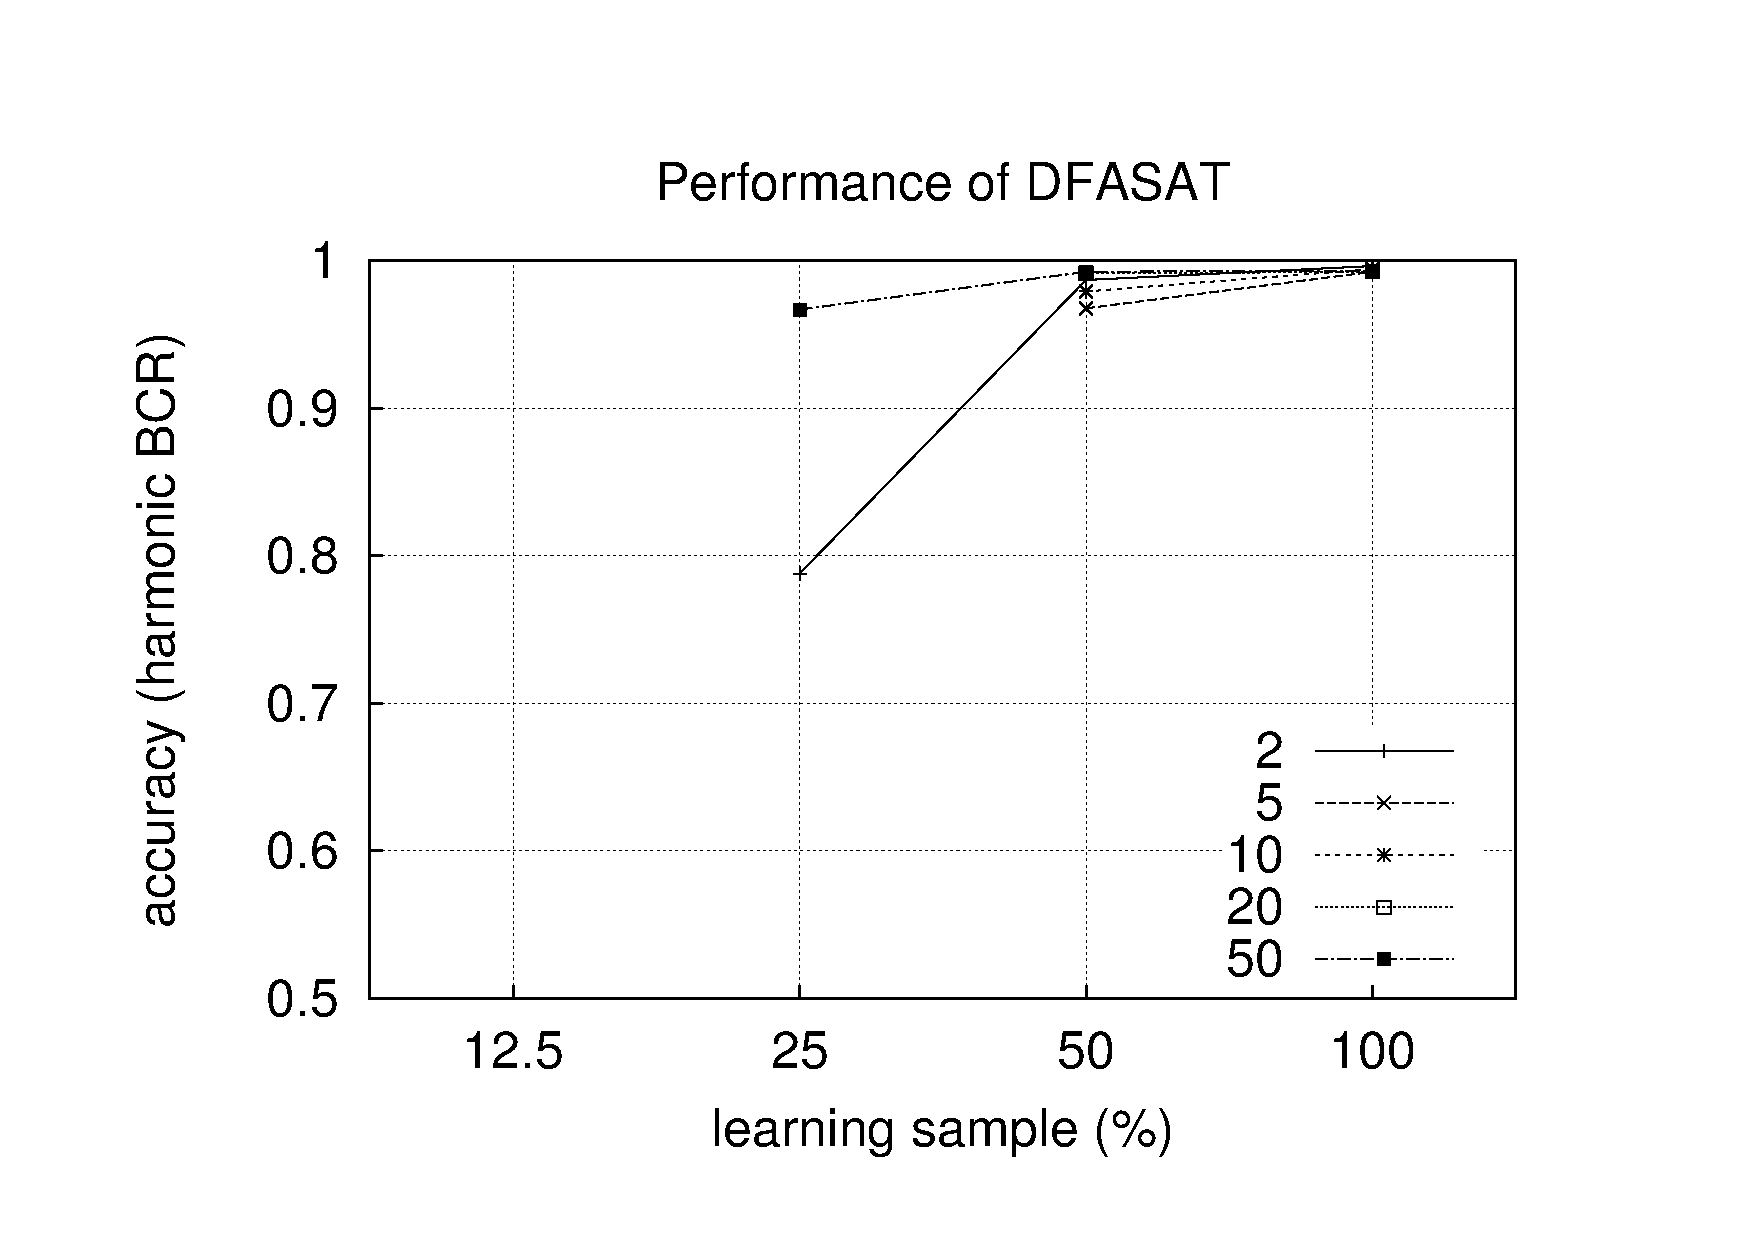
\includegraphics[trim=20mm 0mm 25mm 0mm, clip]{src/6-stamina/images/DFASAT-performance}
  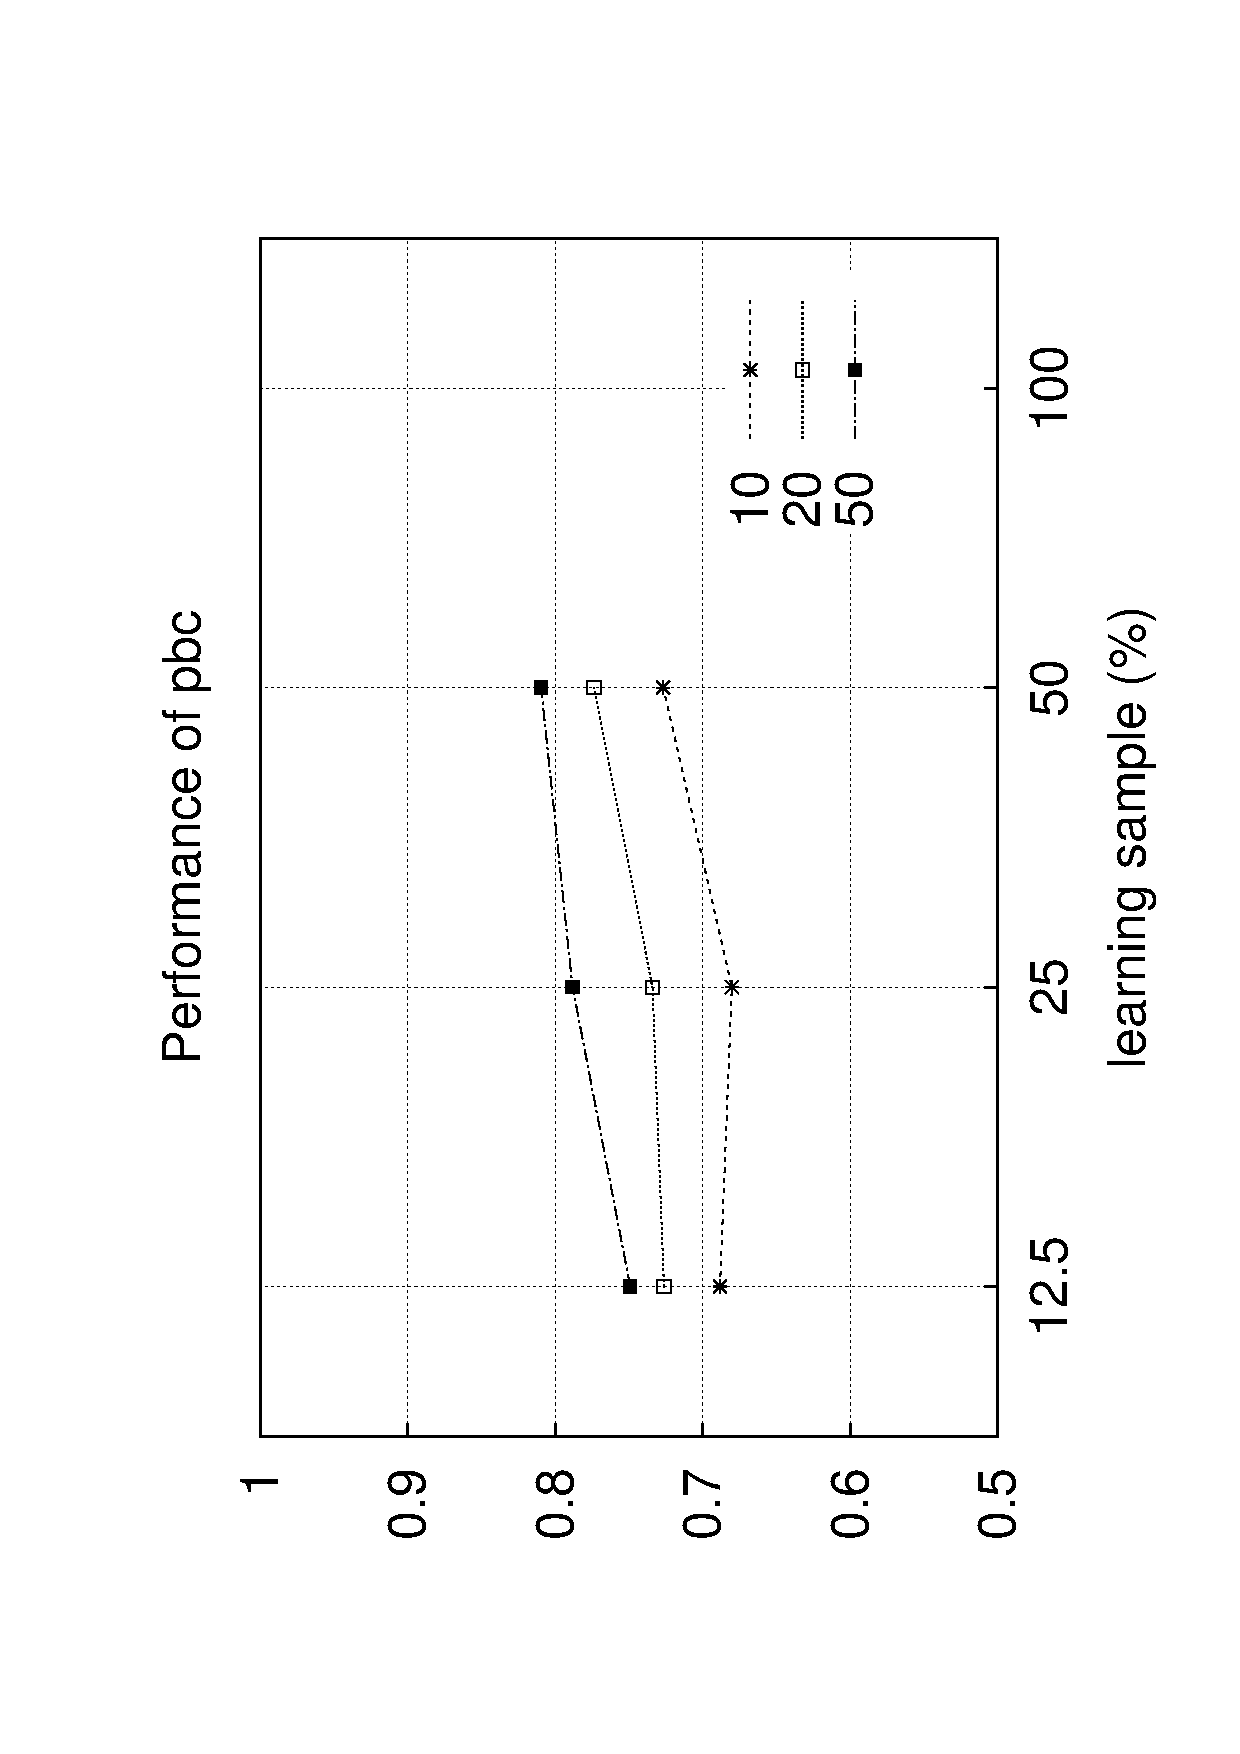
\includegraphics[trim=20mm 0mm 25mm 0mm, clip]{src/6-stamina/images/pbc-performance}}
  \caption{Performance curves of DFASAT and pbc\label{image:stamina-winners-performance-comparison}.}
\end{figure}

In any case, a quick comparison of the curves in Fig.~\ref{image:stamina-winners-performance-comparison} with the baseline curves in Fig.~\ref{stamina:image:bluefringe-performance} perfectly illustrates the overall contribution of the competition and of these two approaches in particular: on the kind of problems considered in Stamina, the state-of-the-art in grammar induction has been pushed significantly forward.

%%%%%%

\section{Evolution toward an evaluation platform\label{section:stamina-platform}}

In the spirit of Abbadingo, the competition website is still available online and aims at becoming an online benchmark for evaluating novel induction techniques. To achieve this goal a few changes have already been made on the competition server:

\begin{itemize}

\item The average score obtained by Blue-fringe on each cell has been published in the documentation section of the website. Also, the cell difficulty level has been made obsolete and is only kept for documentation purposes of the competition itself.

\item The public hall of fame has been updated in a direction similar to what has been discussed in Section~\ref{subsection:stamina-trends-on-hardest-cells}. Indeed, instead of displaying the winners of broken cells only, each cell is annotated with the three best challengers in descending order of their average score for that cell (which is also given). 

\item The oracle has not been modified and still gives a binary feedback only, to continue preventing hill-climbing. However, the private participant section has been updated in a way similar to the hall of fame. Now, the private submission grid displays the average score obtained on each of the cell for which she has submitted.

\end{itemize}

In both cases -- public hall of fame and private section -- having submitted for the five problems of a cell is a necessary condition for results to be taken into account. Imposing such a criteria guarantees sound comparisons between participants. It is also a strong incentive to run a technique on all problems of a given difficulty, partly overcoming the problem of having only partial results available for analyzes that we discussed earlier. These choices have been made with a double objective in mind. The first one is to provide a more transparent feedback in the form of an exact scoring mechanism helping participants to self-evaluate, without being tempted to hijack the oracle (changes in the private section). The second one is to keep a competitive aspect to the platform, which counts in the motivation for using it (implemented by the new hall of fame). 

Future work along a certain number of directions is worth considering, some of them being even required to use the platform to evaluate the techniques of the present thesis:

\begin{itemize}

\item First, interactive inductive techniques (e.g. QSM) could hardly compete so far, due to the absence of an online oracle answering membership queries. While implementing such an oracle does not present particular difficulties (except, maybe, to guarantee scalability in presence of numerous demanding challengers), it would require generating fresh new problems to avoid interfering with the current grid and challengers already competing on it. 

\item White box benchmarks -- where target machines would be disclosed together with samples -- could also be envisaged in order to help evaluating, on a common basis, inductive techniques involving domain information like fluents or mandatory merge constraints. Alternatively, sharing binaries for generating new target machines and samples could help reusing the Stamina protocol. 

\item Last, the protocol used to generate samples (random walks from the machine, noisy perturbation to obtain negative strings and the presence of duplicates in the training set) is an interesting aspect of Stamina, but does not seem to have been used by participants. While it allows tackling the induction problem with statistical approaches, it also triggers a question about the splitting between training and test samples and the impact it could have on the observed frequency of use, in the training set, of each transition of the target. At the time of writing, further study of competition data is still required to answer the question.

\end{itemize}

\section*{Summary}

This chapter presented \emph{Stamina}, an evaluation platform for inductive model synthesis that completes a previous platform from the machine learning community, known as Abbadingo. Key differences with the latter is that Stamina focuses on the difficulty of the learning with respect to the alphabet size and relies on adapted protocols for generating target machines and samples presenting characteristics observed on models used by the software engineering community. Like Abbadingo, Stamina was first designed to be a formal competition in automaton induction. This competition has been won by DFASAT, a novel induction algorithm that significantly pushed forward the state-of-the-art, by outperforming Blue-fringe used as baseline. Among other ingredients, DFASAT identified an alternative scoring heuristics to the one of Blue-fringe that proved very useful for inferring the kind of behavior models proposed. Since the end of the competition, Stamina has evolved to an online benchmark along a certain number of directions. It is available at \verb|http://stamina.chefbe.net|
